\documentclass{beamer}

\usepackage{amsmath}
\usepackage{amssymb}
\usepackage{indentfirst}
\usepackage{graphicx}
\usepackage{subcaption}

\graphicspath{{../../imgs}}
\usetheme{Madrid}


\newcommand{\bld}[1]{\textbf{#1}}

\author{Kainã Alves Tureso}
\title{Simulação de corpos em flutuação}
\date{\today}
\institute{ICMC-USP}




\begin{document}

\frame{\titlepage}
\frame{
    \tableofcontents
}


\section{Equivalência de equilíbrio - Newton/PVI}
\begin{frame}{Equivalência de equilíbrio - Newton/PVI}
    \begin{figure}
        \centering
        % Subfigura 1 - Ocupa 45% da largura do texto
        \begin{subfigure}[b]{0.45\textwidth}
            \centering
            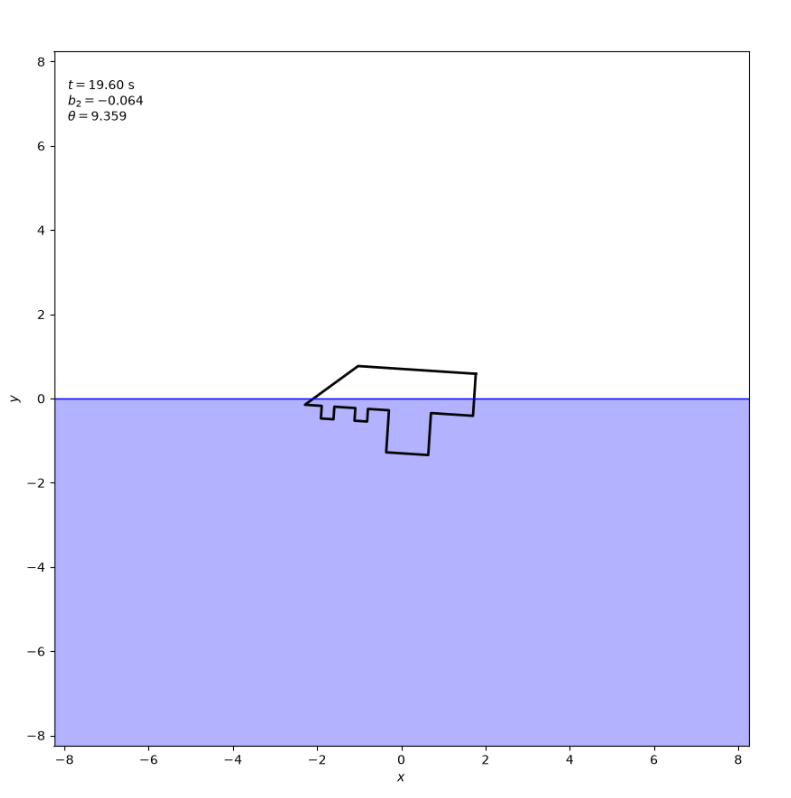
\includegraphics[width=\textwidth]{equi_PVI.png}
            \caption{Equilíbrio no PVI}
        \end{subfigure}
        \hfill % Empurra a segunda imagem para a extremidade direita
        % Subfigura 2 - Ocupa 45% da largura do texto
        \begin{subfigure}[b]{0.45\textwidth}
            \centering
            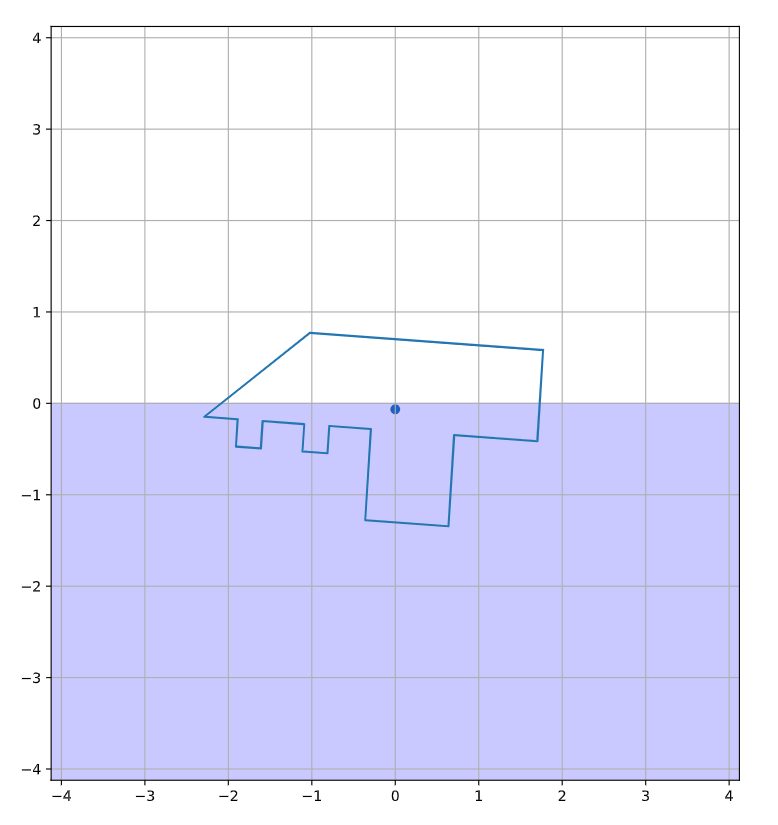
\includegraphics[width=\textwidth]{equi_Newton.png}
            \caption{Equilíbrio em Newton}
        \end{subfigure}
    \end{figure}
\end{frame}



\section{Adaptação do termo difusivo}
\begin{frame}
    \frametitle{PVI}
    Seja $\gamma > 0$ constante. Definimos
    \[
        \textbf{u}(t) = \begin{bmatrix}
            b_2(t) \\
            b_2'(t) \\
            \theta(t) \\
            \theta'(t)
        \end{bmatrix} = \begin{bmatrix}
            u_0 \\ u_1 \\ u_2 \\ u_3
        \end{bmatrix}
    \] \pause

    e

    \[
        \bld{u}'(t) = \bld{f}(\bld{u}(t), t) = \begin{bmatrix}
            u_1\\
            \frac{1}{m}(F_1(u_2, u_0) - \gamma V u_1) \\
            u_3 \\
            \frac{1}{I}(F_2(u_2, u_0) - \gamma I u_3)
        \end{bmatrix}
    \]
\end{frame}

\begin{frame}
    \frametitle{Tratamento do termo difusivo}
    Originalmente, tínhamos $\gamma > 0$ constante. Fisicamente isso pode ser um problema, principalmente quando o corpo está completamente fora do líquido. \pause
    

    O que fazer? \pause

    Podemos fazer $\gamma$ variar na proporção do corpo que está submersa. Note que, como a densidade do objeto é constante, temos que $E = \rho_L  g  V_f$, em que $\rho_L$ é a densidade do líquido, $V_f$ é o volume de líquido deslocado e $g$ é a aceleração gravitacional. Com isso, o volume submerso é $V_f = E / (\rho_L  g)$.
    Definimos então $\gamma_f = \gamma \frac{V_f}{V}$
\end{frame}

\begin{frame}
    Obtemos então a seguinte adaptação da $\bld{f}$:
    \[
        \bld{f}(\bld{u}(t), t) = \begin{bmatrix}
            u_1\\
            \frac{1}{m}(F_1(u_2, u_0) - \gamma V_f u_1) \\
            u_3 \\
            \frac{1}{I}(F_2(u_2, u_0) - \gamma_f I u_3)
        \end{bmatrix}
    \]
\end{frame}




\section{Análise de convergência}
\begin{frame}
    \frametitle{Escolha do tamanho de passo}
    Utilizando o objeto "cow" com densidade $\rho = 0.5$, densidade da água $\rho_L = 1.0$, $\gamma = 0.7$ e $\bld{u}_0 = (6.0, 0.0, 0.0, 3.0)$ obtemos a seguinte figura:
    \begin{figure}
        \centering
        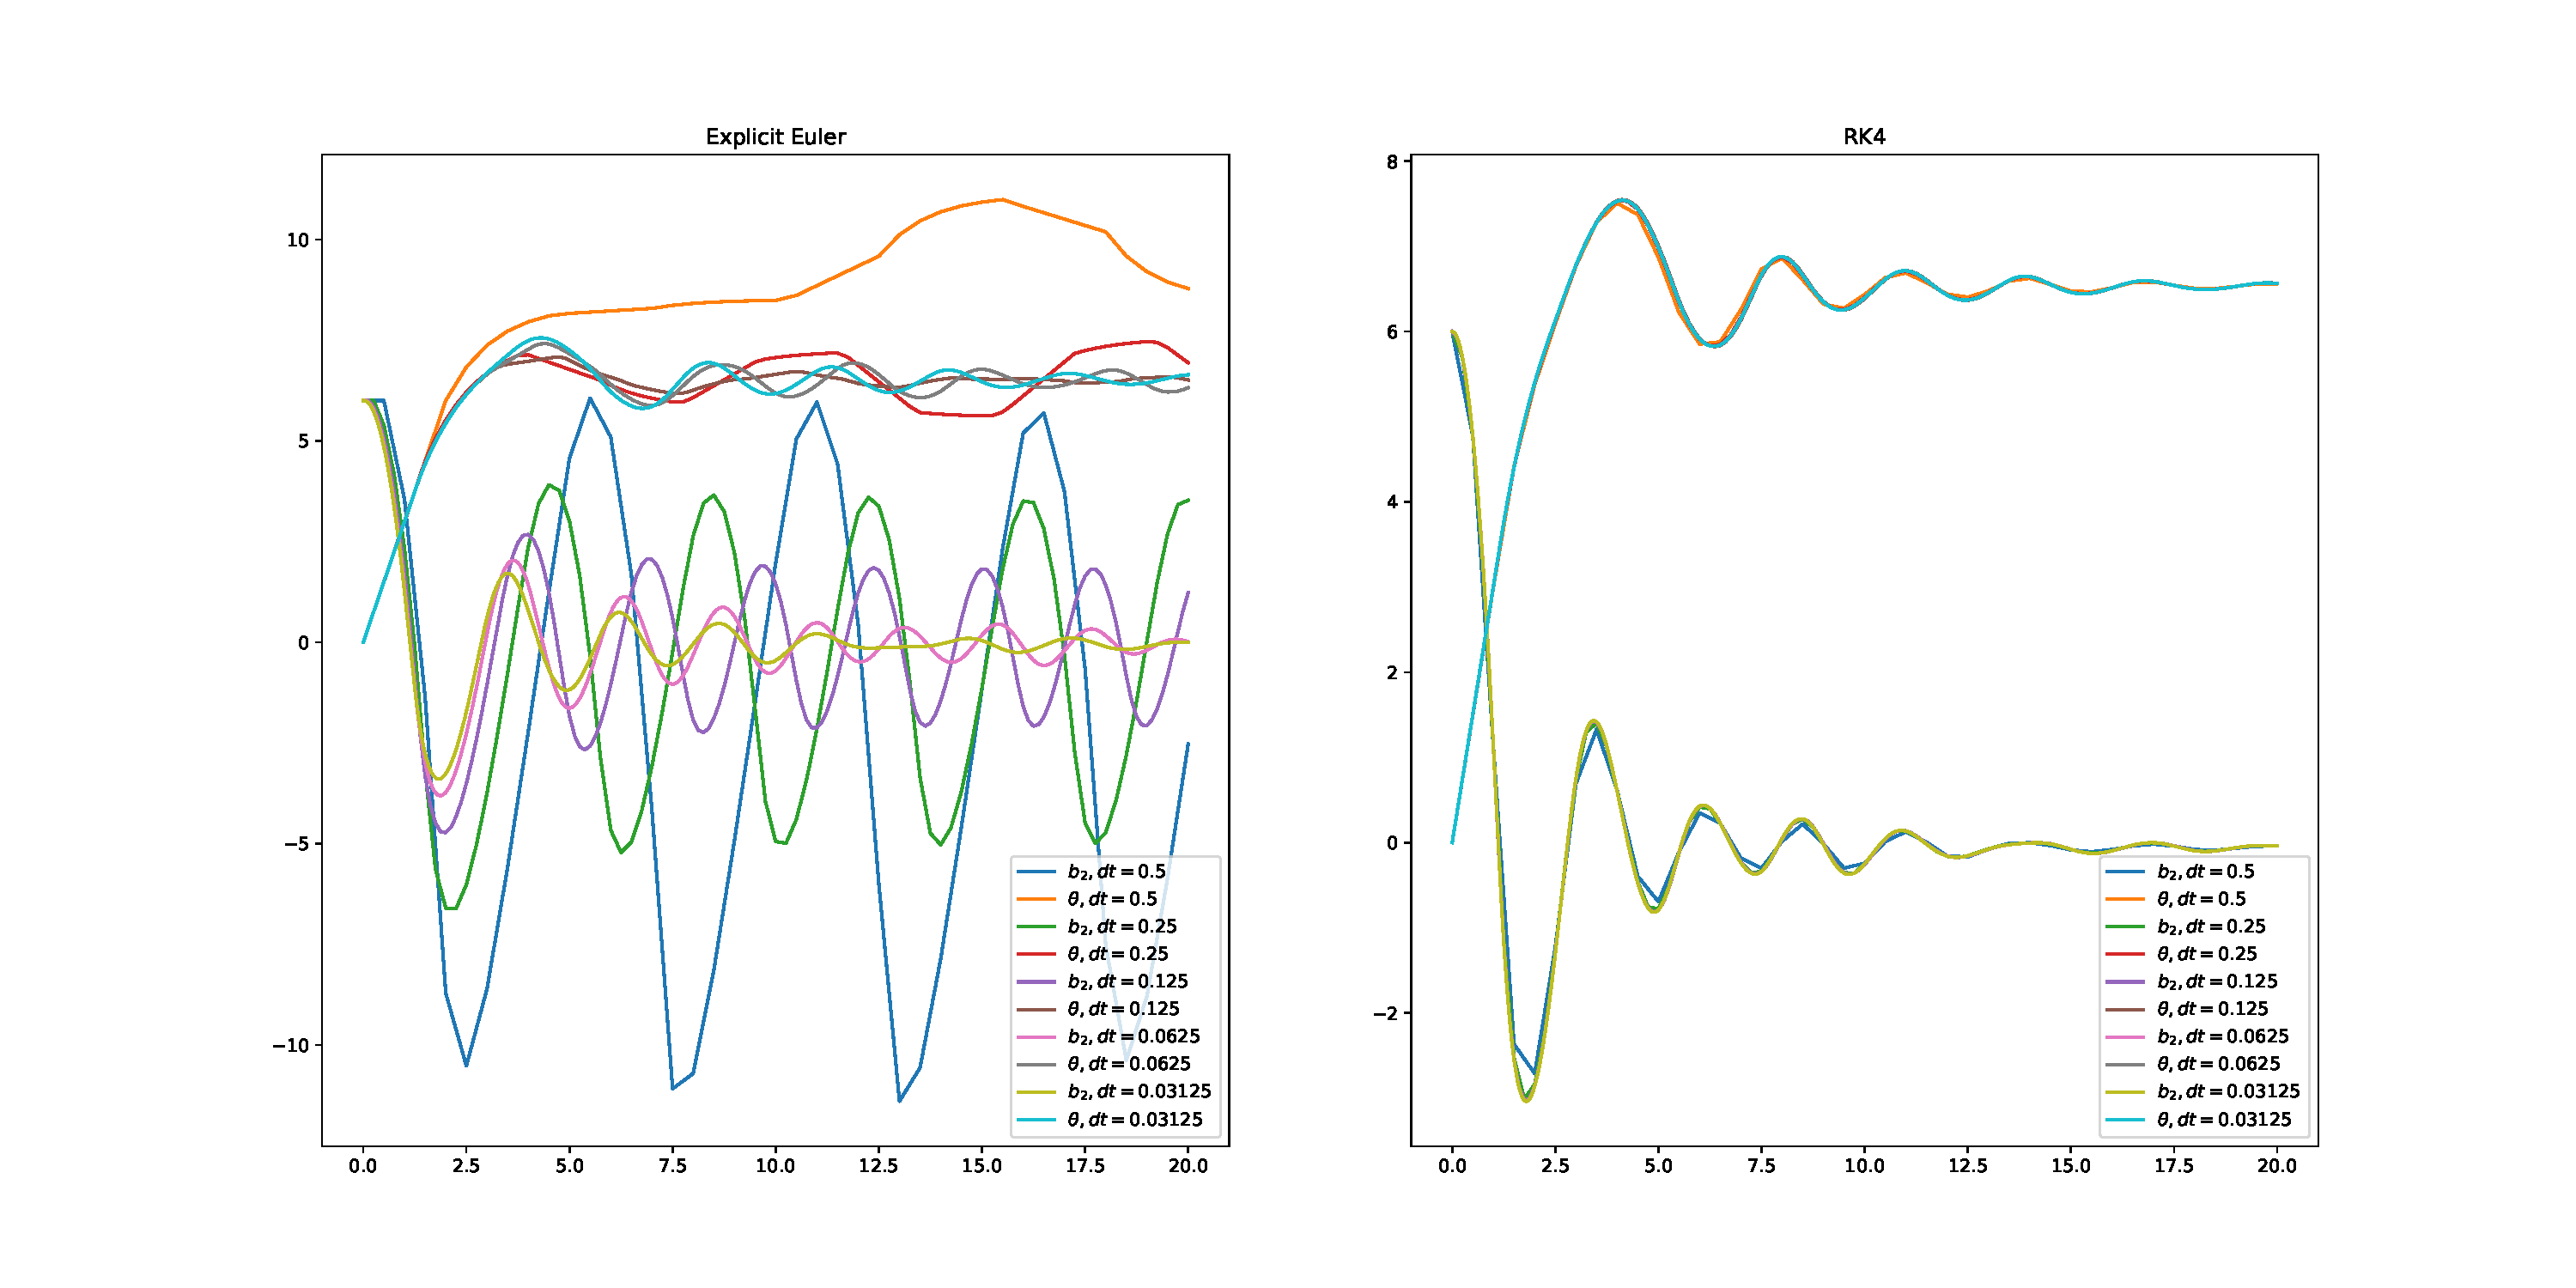
\includegraphics[width=0.8\textwidth]{cow_PVI_conv.pdf}    
        \caption{Solução do PVI com diferentes passos de tempo. Euler explícito na esquerda, Runge-Kutta 4 na direita}
        \label{fig:PVI_time}
    \end{figure}
\end{frame}

\begin{frame}
    Os métodos aparentam ter ordem de convergência menor que a esperada, considerando a norma $L^2$ discreta.
    \begin{figure}
        \centering
        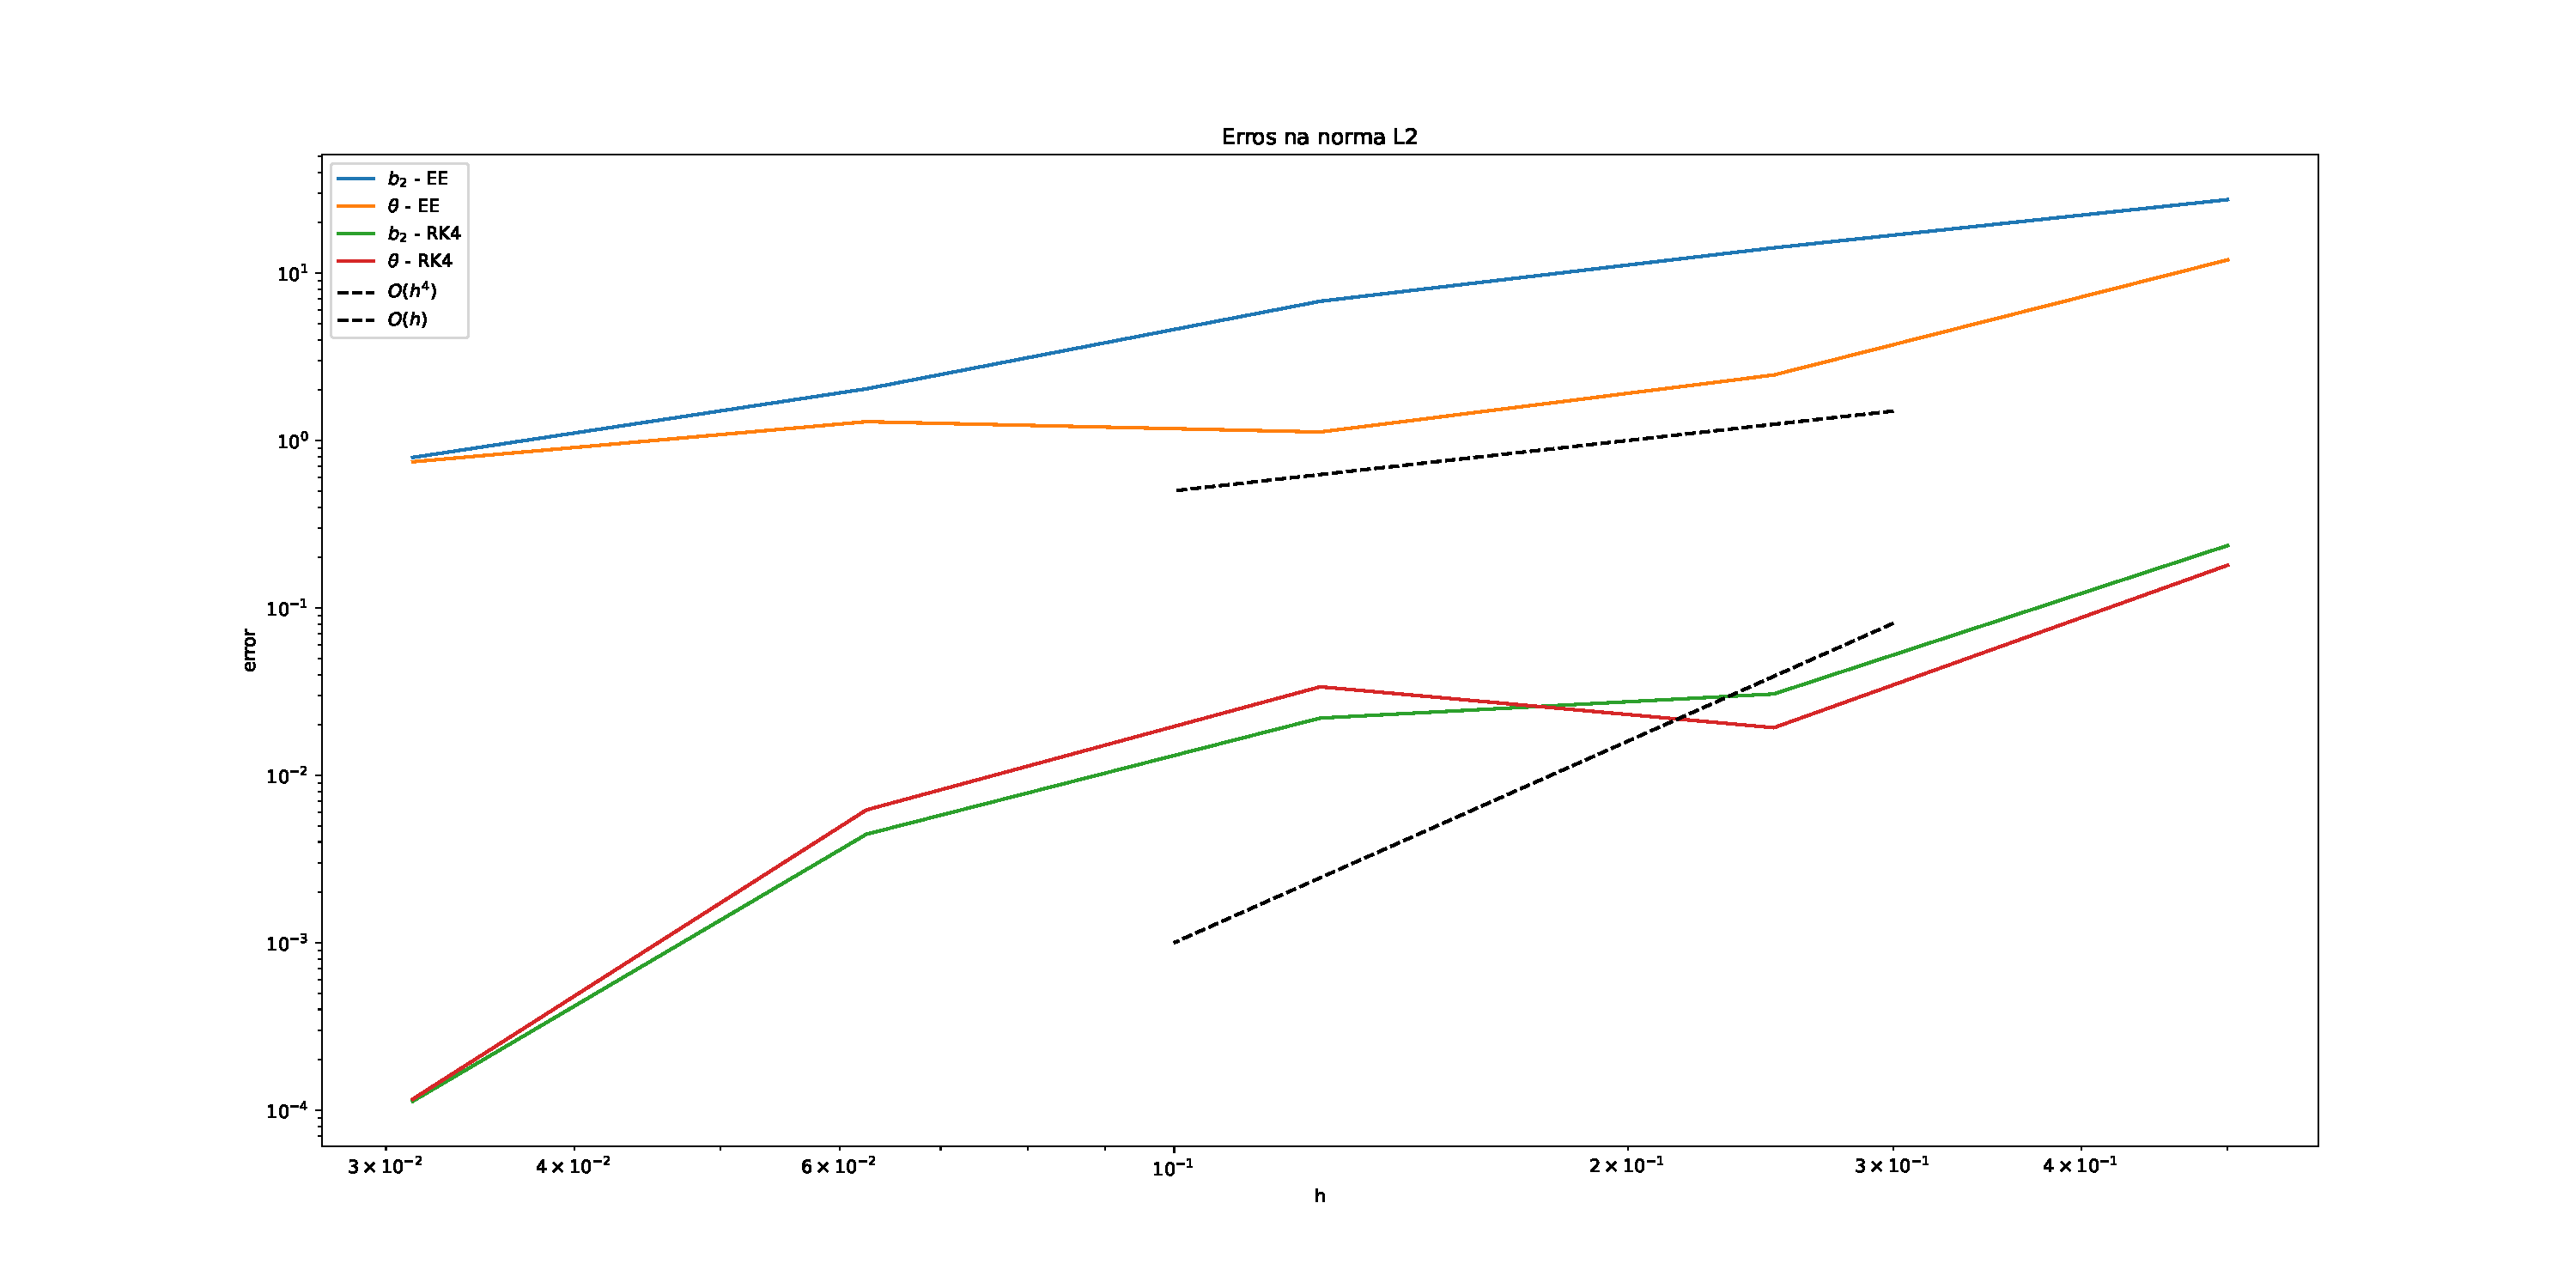
\includegraphics[width=0.9\textwidth]{cow_PVI_conv2.pdf}
        \caption{Erros na norma $L^2$}
        \label{fig:L2}
    \end{figure}
\end{frame}

\end{document}